%
% geometry.tex -- Geometry of QLPDE 1rd order
%
% (c) 2019 Prof Dr Andreas Mueller
%
\chapter{Geometry of partial differential equations of first order%
\label{chapter:geometry}}
\lhead{Geometry of solutions}
\begin{figure}
\begin{center}
\includegraphics[width=\hsize]{../common/images/ode-1.pdf}
\end{center}
\caption{direction field of the ordinary differential equation 
$y'=-\frac16y+e^{-\frac{x}6}\cos x$ \label{geometrie:ode}}
\end{figure}
The direction field of an ordinary differential equation is a very
\index{direction field}
convenient way to build an intuition about the solutions of an equation
(figure~\ref{geometrie:ode}).
The solution curve is tangent to directions specified by the differential
equation.


The solution of a partial differential equation with two independent
variables, which is the situation we will restrict ourselves to in
this chapter, can be visualized as a surface.
Is there a concept similar to the direction field of an ordinary
differential equation that helps us visualize the solutions?
The first idea that comes to mind is a field of tangent planes.
\index{tangent plane}
Such a field would fix the first derivatives individually.
What a partial differential equation does, however, is to only fix an
often linear combination of first derivatives.
We have to accept a more complicated answer.

%
% geometrie.tex %% Beispiele partieller Differentialgleichungen -- XXX
%
% (c) 2008 Prof Dr Andreas Mueller
%
\begin{figure}
\centering
\begin{tabular}{cc}
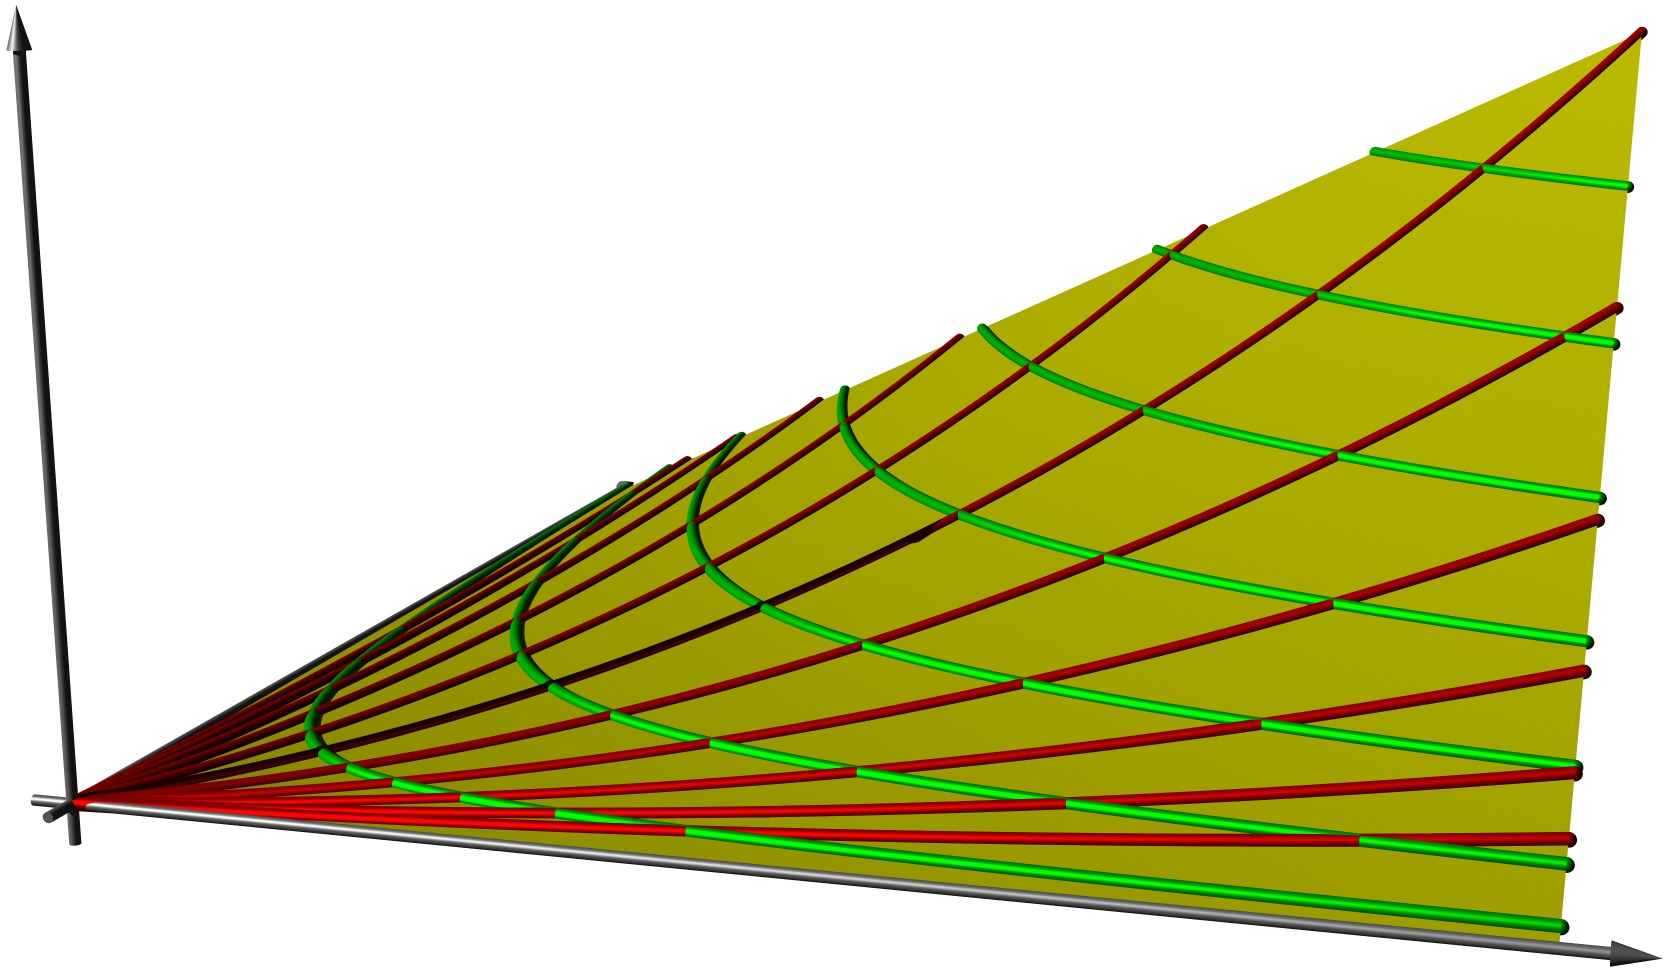
\includegraphics[width=0.6\hsize]{../common/3d/surface.jpg}&%
\includegraphics[width=0.35\hsize]{../common/images/kurven-1.pdf}
\end{tabular}
\caption{Die Fläche, die als Graph $z=f(x,y)$ der Funktion $f(x,y)=xy$
dargestellt werden kann, kann auch als Vereinigung der roten oder grünen
Kurvenscharen beschreiben werden.
Die Fläche kann auch mit der Parameterdarstellung
\eqref{quasliniear:flaechebeispiel}
dargestellt werden.
Die grünen Kurven sind die Koordinatenlinien dieser Parameterdarstellung
mit $s=\operatorname{const}$,
die roten Kurven sind Koordinatenlinien mit $t=\operatorname{const}$.
Links im Bild die Darstellung als Fläche, rechts die Koordinatenlinien
${\color{red}t}=\operatorname{const}$
und
${\color{green}s}=\operatorname{const}$
im Grundriss.
\label{quasilinear:flaechenalskurven}
}
\end{figure}

\section{Kurven auf der Lösungsfläche}
\rhead{Kurven auf der Lösungsfläche}
Die Lösungsfläche ist unausweichlich ein zweidimensionales
Objekt, dem nur mit partiellen Ableitungen beizukommen ist.
Die einzige Möglichkeit, das Problem auf eine gewöhnliche
Differntialgleichung zu reduzieren besteht darin, die Lösungsfläche
``kurvenweise'' zu finden, sie also eine Schar von Kurven
zu betrachten.

\subsubsection{Lösungsfläche als Kurvenschar}
Der Graph der Funktion $u(x,y)$ kann auf zwei Arten als Schar von
Kurven betrachtet werden.
Einerseits als durch die Werte $y$
parametrisierte Schar von Kurven $x\mapsto u(x,y)$, andererseits
also durch Werte $x$ parametrisierte Schar von Kurven $y\mapsto u(x,y)$.
Allerdings könnte auch jede andere Parametrisierung der Fläche
zu so einer Zerlegung Anlass geben. Die Parametrisierung
\begin{equation}
(s,t)\mapsto \vec x(s,t)
=
\begin{pmatrix}x(s,t)\\y(s,t)\\z(s,t)\end{pmatrix}
\label{quasilinear:kurvenschar}
\end{equation}
liefert die durch $s$ parametrisierte Schar $t\mapsto \vec x(s,t)$
von Kurven und die durch $t$ parametrisierte Schar $s\mapsto\vec x(s,t)$.

In Abbildung~\ref{quasilinear:flaechenalskurven} ist der Graph der
Funktion $u(x,y)=xy$ dargestellt.
Man kann ihn auch mit den Parametern $t$ und $s$ gemäss
\begin{equation}
(t,s)
\mapsto
\begin{pmatrix}x\\y\\z\end{pmatrix}
=
\begin{pmatrix}t\sqrt{s}\\\frac1t\sqrt{s}\\s\end{pmatrix}
\label{quasliniear:flaechebeispiel}
\end{equation}
parametrisieren.
Tatsächlich gilt $xy = t\sqrt{s}\frac1t\sqrt{s}=s=z$.
Die resultierenden Kurvenscharen sind in
Abbildung~\ref{quasilinear:flaechenalskurven} als rote und grüne Kurven
dargestellt.

Umgekehrt beschreibt eine Schar von Kurven eine Fläche, die sich
in vielen Fällen wieder als Funktion $u(x,y)$ schreiben lassen wird.
Man muss dazu nur für jeden Punkt $(x,y)$ die Gleichungen
\begin{align*}
x(s(x,y),t(x,y))&=x\\
y(s(x,y),t(x,y))&=y
\end{align*}
lösen.
Die so bestimmten Funktionen $s(x,y)$ und $t(x,y)$ setzt man dann in
die Funktion $z(x,y)$ ein, und erhält die
Lösungsfunktion
\[
u(x,y)=z(s(x,y), t(x,y)).
\]
Das Ziel ist also, eine Schar (\ref{quasilinear:kurvenschar})
von Kurven zu finden, die alle auf der Lösungsfläche liegen.

\begin{beispiel}
\begin{figure}
\centering
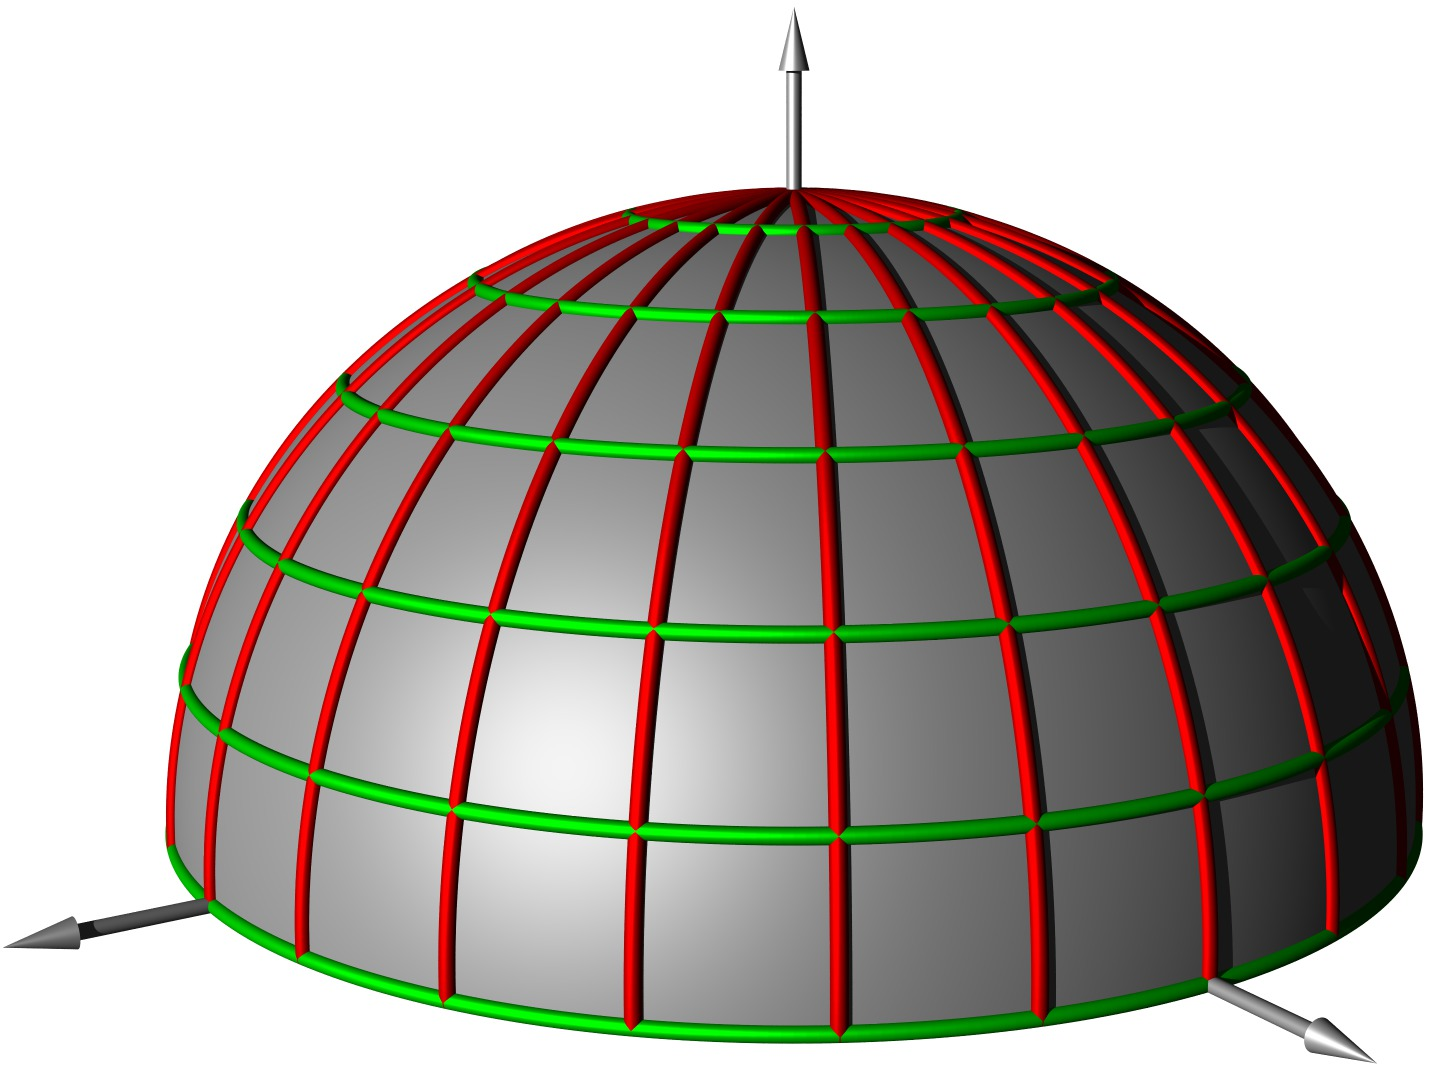
\includegraphics[width=0.8\hsize]{../common/3d/kugel.jpg}
\caption{Darstellung der Halbkugel als Vereinigung zweier Kurvenscharen
\label{quasilinear:kugel}}
\end{figure}
Die Parametrisierung
\[
(\vartheta,\varphi)\mapsto
\begin{pmatrix}
\sin\vartheta\cos\varphi\\
\sin\vartheta\sin\varphi\\
\cos\vartheta
\end{pmatrix}
\]
beschreibt für $0\le \vartheta\le \frac{\pi}2$
und $0\le\varphi\le 2\pi$ eine Halbkugel (Abbildung~\ref{quasilinear:kugel}).

Die Kurvenscharen
\[
\vartheta\mapsto
\begin{pmatrix}
\sin\vartheta\cos\varphi\\
\sin\vartheta\sin\varphi\\
\cos\vartheta
\end{pmatrix}
\qquad
\text{und}
\qquad
\varphi\mapsto
\begin{pmatrix}
\sin\vartheta\cos\varphi\\
\sin\vartheta\sin\varphi\\
\cos\vartheta
\end{pmatrix}
\]
sind die durch $\varphi$, die geographische Länge, parametrisierten
Längen- und die durch $\vartheta$, die geographische Breite
parametrisierten Breitenkreise auf der Kugeloberfläche.

Die Gleichungen
\begin{align*}
x&=\sin\vartheta\cos\varphi\\
y&=\sin\vartheta\sin\varphi\\
\end{align*}
lassen sich mindestens für $x\ne 0$ durch
\begin{align*}
\tan\varphi&=\frac{y}{x}\\
\sin\vartheta &=\sqrt{x^2+y^2}
\end{align*}
auflösen. Dies reicht bereits, um die Funktion $u(x,y)$
auszudrücken:
\[
u=\cos\vartheta=\sqrt{1-\sin^2\vartheta}=\sqrt{1-x^2-y^2}.
\qedhere
\]
\end{beispiel}

\subsubsection{Erster Parameter: Cauchy-Anfangswerte}
\begin{figure}
\begin{center}
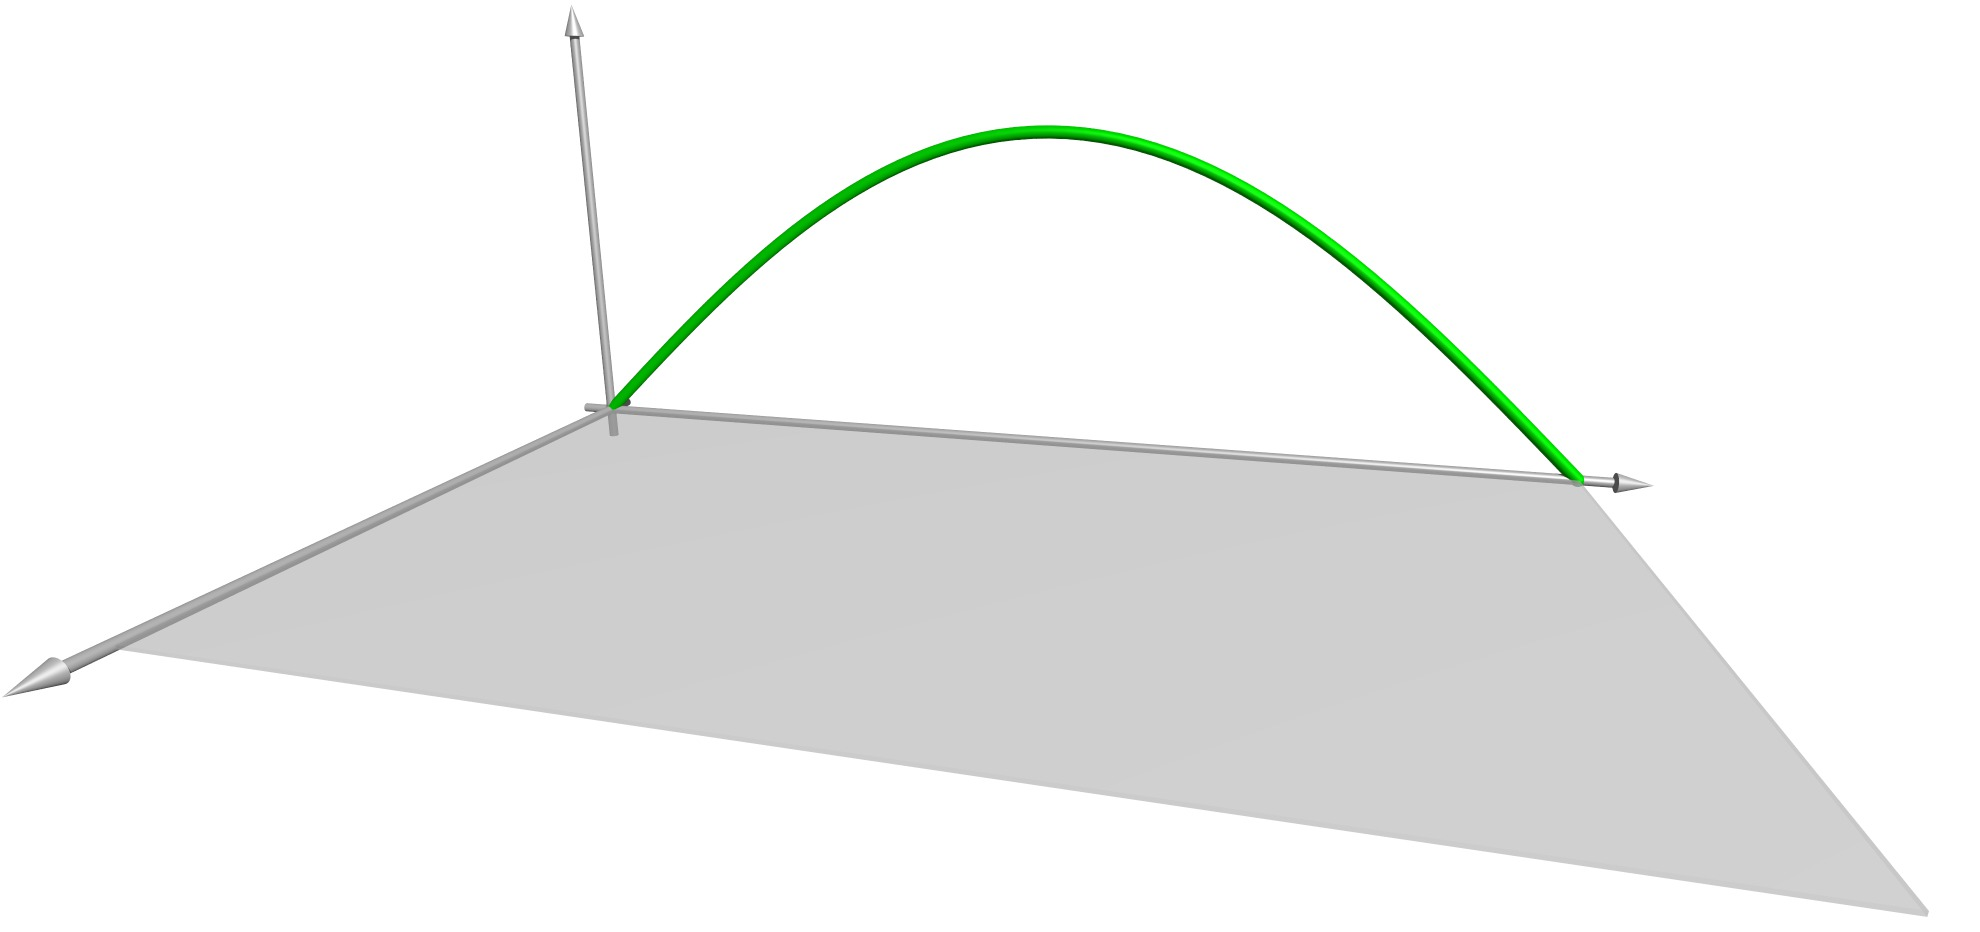
\includegraphics[width=\hsize]{../common/3d/cauchy.jpg}
\end{center}
\caption{Cauchy-Anfangskurve für eine partielle Differentialgleichung
($y$-Achse nach rechts)
\label{geometrie:cauchy-anfangskurve}}
\end{figure}
Wir wollen für partielle Differentialgleichungen erster Ordnung
das Cauchy-Problem lösen.
Das bedeutet, dass eine Anfangskurve bereits vorgegeben ist
(Abbildung~\ref{geometrie:cauchy-anfangskurve}).
Es gibt also eine Kurve
\begin{equation}
s\mapsto\vec x_0(s)=\begin{pmatrix}
x_0(s)\\
y_0(s)\\
z_0(s)
\end{pmatrix},
\label{quasilinear:anfangskurve}
\end{equation}
und die gesuchte Lösungsfunktion $u(x,y)$ muss für jedes $s$ die
Bedingung
\[
u(x_0(s), y_0(s))=z_0(s)
\]
erfüllen.
Man muss diese Kurve jetzt also erweitern zu einer Kurvenschar
der Form (\ref{quasilinear:kurvenschar}).
Für $t=0$ muss die Anfangskurve entstehen:
\[
\vec x(s,0)=x_0(s).
\]
Jede Scharkurve $t\mapsto \vec x(s,t)$ ist also eine Kurve
mit Anfangspunkt $x_0(s)$.
Es liegt nahe, solche Scharkurven als Lösungen von gewöhnlichen
Differentialgleichungen zu finden.

\subsection{Quasilineare partielle Differentialgleichung erster Ordnung}
Wir betrachten in diesem Abschnitt eine quaslineare partielle 
Differentialgleichung
\begin{equation}
a\frac{\partial u}{\partial x}
+
b\frac{\partial u}{\partial y}
=
c.
\label{quasilinear:equation}
\end{equation}
Wir wollen zeigen, dass für diese Art von Differentialgleichungen
das Cauchy-Problem meistens lösbar ist, und wollen verstehen,
unter welchen Bedingungen es nicht lösbar ist.

\subsubsection{Gewöhliche Differentialgleichung erster Ordnung}
Wir erinnern uns zunächst an die Lösung der gewöhnlichen
Differentialgleichungen erster Ordnung.
Eine solche legt die Ableitung $y'$ in Abhängigkeit von 
$(x,y)$ durch eine Funktion $f(x,y)$ fest: 
\[
y'=f(x,y).
\]
Gesucht ist dann eine Kurve $y(x)$, welche
in jedem Punkt $x$ die Steigung $y'(x)=f(x,y(x))$.
Geometrisch legt die Funktion $f(x,y)$ ein Richtungsfeld fest,
der Graph der Lösung ist eine Kurve, deren Tangente in jedem
Punkt mit dem Richtungsfeld zusammenfällt.

Um eine Lösungskurve zu finden, kann man wie folgt vorgehen.
Die Anfgangswerte  $y(0)=y_0$ legen einen Punkt fest.
Die Differentialgleichung liefert jetzt die Steigung in
diesem Punkt: $y'(0)=f(0,y(0))$.
In erster Näherung ist daher
\begin{equation}
y(h)=y(0)+f(0,y(0))\cdot h.
\label{quasilinear:euler}
\end{equation}
Mit $y(h)$ können wir das Verfahren wiederholen, und durch
wiederholte Anwendung von (\ref{quasilinear:euler})
nacheinander $y(2h)$, $y(3h)$,\dots bestimmen.
Natürlich ist dies nur ein Näherungsverfahren, das übrigens
von Euler erdacht worden ist. Macht man $h$ sehr klein, wird
die Approximation der wahren Lösung immer besser.
Aber es macht plausibel, warum eine gewöhnliche Differentialgleichung
erster Ordnung genau eine Anfangsbedingung braucht.

\subsubsection{Lösbarkeit}
Wir versuchen jetzt, diese Überlegung auf die Lösbarkeit einer
Differentialgleichung der Form (\ref{quasilinear:equation}) zu 
übertragen.
Wir haben jetzt natürlich zwei partielle Ableitungen, die
durch die Gleichung (\ref{quasilinear:equation}) auch nicht
eindeutig bestimmt sind.
Als lineare Gleichung für die partiellen
Ableitungen betrachtet, hat (\ref{quasilinear:equation}) unendlich 
viele Lösungen.

Dies ist allerdings nicht so schlimm: denn wir möchten ja das Cauchy-Problem
lösen: vorgegeben sind die Werte der Funktion entlang einer Kurve.
Wir haben also auch unendlich viele ``Anfangswerte''.
Zur Vereinfachung der Diskussion nehmen wir zunächst an, dass die
Funktionswerte für $x=0$ vorgegeben sind.
Damit sind aber nicht nur die Funktionswerte $u(0,y)$ bekannt, sondern
auch die partiellen Ableitungen $\partial_yu(0,y)$.

Wenn der Koeffizient $a(x,y,u)$
in (\ref{quasilinear:equation})
von $0$ verschieden ist, kann man die Gleichung
nach $\partial_xu$ auflösen.
Die eine partielle Ableitung legt also die andere fest.
Durch die Anfangswerte ist die eine partielle Ableitung auf der
Anfangskurve bereits festgelegt, nämlich die entlang der Anfangskurve,
also steht auch die andere Ableitung schon fest.

Wir sind also in einer ähnlichen Situation wie bei gewöhnlichen
Differentialgleichungen erster Ordnung: Wenn wir die 
Anfangskurve zum Beispiel für $x=0$ kennen, also Werte
$u(0,y)$ bereits kennen, dann kennen wir
auch die Ableitungen, und können damit die Lösung
$y\mapsto u(h, y)$ für ein kleines $h>0$ berechnen. Dies legt aber
wiederum die Ableitungen fest, so dass wir noch einen Schritt 
weiter zu $y\mapsto u(2h,y)$ gehen können sollten.
Indem wir so immer weiter schreiten, bekommen wir die ganze
Lösungsfunktion $u(x,y)$.

Wir erwarten daher, dass eine quasilineare partielle Differentialgleichung
nicht schwieriger zu lösen ist, als eine gewöhnliche Differentialgleichung
erster Ordnung.

\subsubsection{Vektorschreibweise der Differentialgleichung}
Die Lösung wird durch die folgende geometrische Überlegung vereinfacht.
Wir stellen dazu die gesuchte Lösungsfunktion $u(x,y)$ als Graph
in einem dreidimensionalen Koordinatensystem $x,y,u$ dar.
Die partielle Differentialgleichung (\ref{quasilinear:equation})
kann auch als Vektorgleichung
\begin{equation}
\begin{pmatrix}a\\b\\c\end{pmatrix}
\cdot
\begin{pmatrix}
\frac{\partial u}{\partial x}\\
\frac{\partial u}{\partial y}\\
-1
\end{pmatrix}
=0.
\label{quasilinear:vektorform}
\end{equation}
geschrieben werden, wie man sich durch Ausmultiplizieren überzeugen
kann.
Den linken Vektor bezeichnen wir mit
\[
\vec v=\begin{pmatrix}
a(x,y,u)\\
b(x,y,u)\\
c(x,y,u)
\end{pmatrix}.
\]
Der rechte Vektor
\[
\vec n=
\begin{pmatrix}
\frac{\partial u}{\partial x}\\
\frac{\partial u}{\partial y}\\
-1
\end{pmatrix}
\]
ist eine Normale auf den Graphen der Funktion
$z=u(x,y)$. Man kann sich von dieser Tatsache zum Beispiel so 
überzeugen: Die Tangentialvektoren in Achsrichtung sind
\[
\vec t_x
=
\begin{pmatrix}1\\0\\\frac{\partial u}{\partial x}\end{pmatrix}
\qquad
\text{und}
\qquad
\vec t_y
=
\begin{pmatrix}0\\1\\\frac{\partial u}{\partial y}\end{pmatrix}
\]
Das Skalarprodukt von $\vec n$ mit den Vektoren $\vec t_x$ und $\vec t_y$
ist:
\[
\vec n\cdot\vec t_x
=
\begin{pmatrix}
\frac{\partial u}{\partial x}\\
\frac{\partial u}{\partial y}\\
-1
\end{pmatrix}
\cdot
\begin{pmatrix}1\\0\\\frac{\partial u}{\partial x}\end{pmatrix}
=0
\qquad
\text{und}
\qquad
\vec n\cdot\vec t_y
=
\begin{pmatrix}
\frac{\partial u}{\partial x}\\
\frac{\partial u}{\partial y}\\
-1
\end{pmatrix}
\cdot
\begin{pmatrix}0\\1\\\frac{\partial u}{\partial y}\end{pmatrix}
=0.
\]
\begin{figure}
\begin{center}
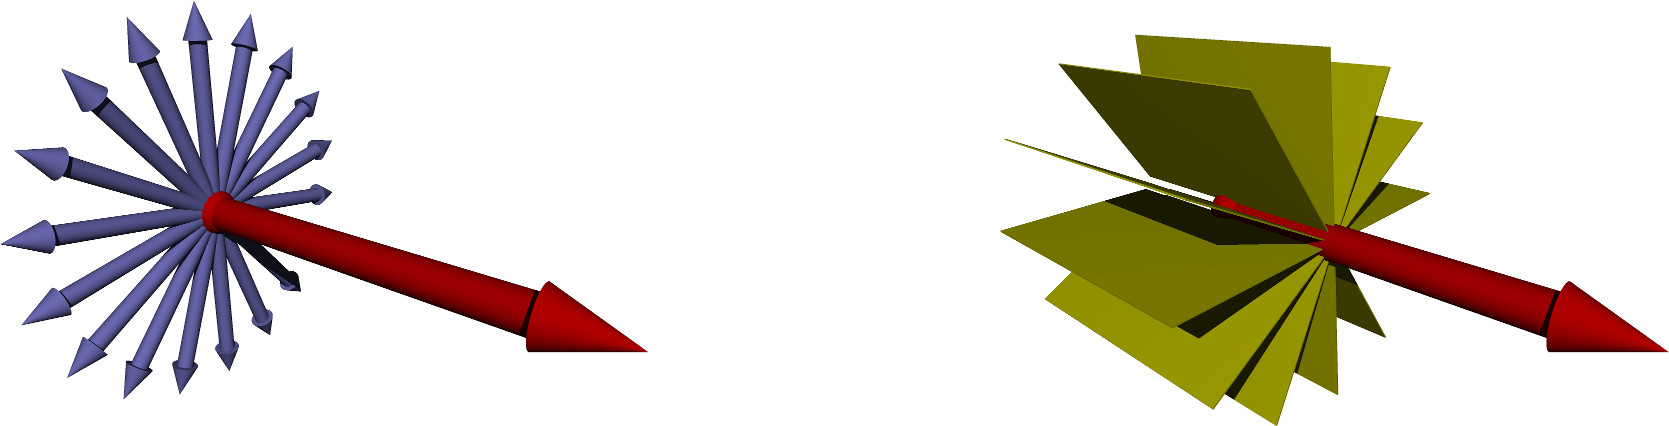
\includegraphics[width=\hsize]{../common/3d/normals.jpg}
\end{center}
\caption{Die Normalen der Lösungsfläche einer quasilinearen
partiellen Differentialgleichung erster Ordnung sind alle senkrecht
auf dem Vektor $\vec v$ (rot, linkes Bild). Die Tangentialebenen an
die Lösungsfläche haben daher eine gemeinsame Gerade mit Richtung $\vec v$.
\label{geometrie:normals}}
\end{figure}%
Die Gleichung (\ref{quasilinear:vektorform}) sagt also,
dass diese Normale senkrecht auf dem Vektor $\vec v$ steht.
Gesucht ist also eine Fläche, deren Normale senkrecht auf dem
Vektor $\vec v$ steht. Die möglichen Tangentialebenen von Lösungen
haben also die Gerade mit Richtung $\vec v$ gemeinsam
(Abbildung~\ref{geometrie:normals}).
Sie bilden ein Büschel von Ebenen.

Wir verstehen jetzt, wie wir das Bild, das wir uns von den gewöhnlichen
Differentialgleichungen gemacht haben, für partielle Differentialgleichungen
modifizieren müssen. Die Differentialgleichung gibt in jedem Punkt
des Raumes ein Büschel von Ebenen vor, welche als Tangentialebenen der
Lösungsfläche in Frage kommen. Die Richtung der Anfangskurve wählt aus
diesem Büschel eine Tangentialebene aus, die Tangentialebene in einem 
Punkt der Anfangskurve muss die Tangente der Anfangskurve enthalten
\begin{figure}
\begin{center}
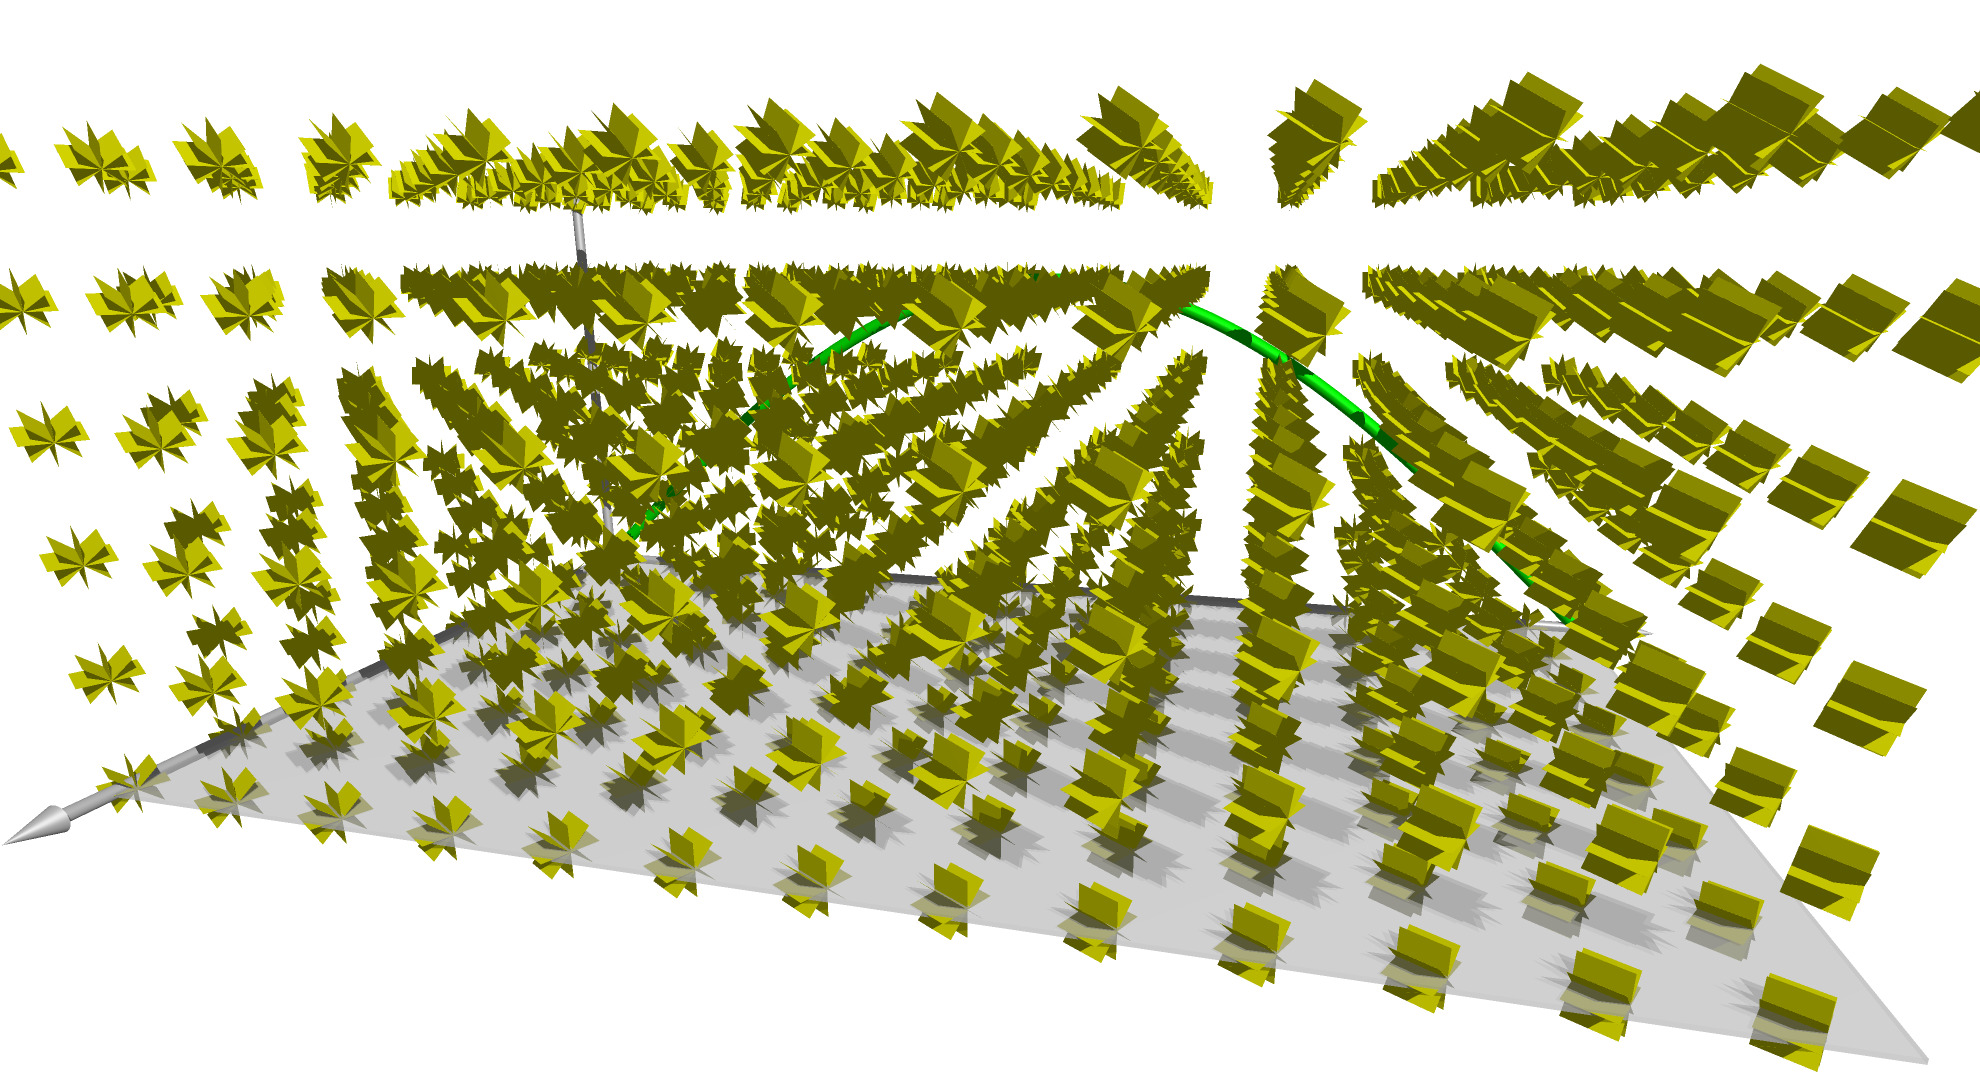
\includegraphics[width=\hsize]{../common/3d/planes.jpg}
\end{center}
\caption{Feld von Ebenenbüscheln, definiert durch eine quasilineare
partielle Differentialgleichung erster Ordnung
\label{geometrie:ebenenbueschelfeld}}
\end{figure}
(Abbildung~\ref{geometrie:ebenenbueschelfeld}).

Das bedeutet zum Beispiel auch, dass die Schnittkurve von
zwei Lösungsflächen immer $\vec n$ als Tangente haben muss.
Kurven, die in jedem Punkt die Richtung $\vec n$ haben, sind
als von ganz besonderer Bedeutung.
Die Vektoren
\[
(x,y,u)\mapsto
\vec v=
\begin{pmatrix}
a(x,y,u)\\b(x,y,u)\\c(x,y,u)
\end{pmatrix}
\]
bilden ein Vektorfeld, welches in jedem Punkt tangential
an die gesuchte Fläche verläuft.

\subsubsection{Charakteristiken}
Statt direkt die Lösungsfläche zu suchen, können wir das Vektorfeld
$\vec v$ dazu verwenden, einzelne Kurven in der Lösungsfläche
zu bestimmen.
\begin{figure}
\begin{center}
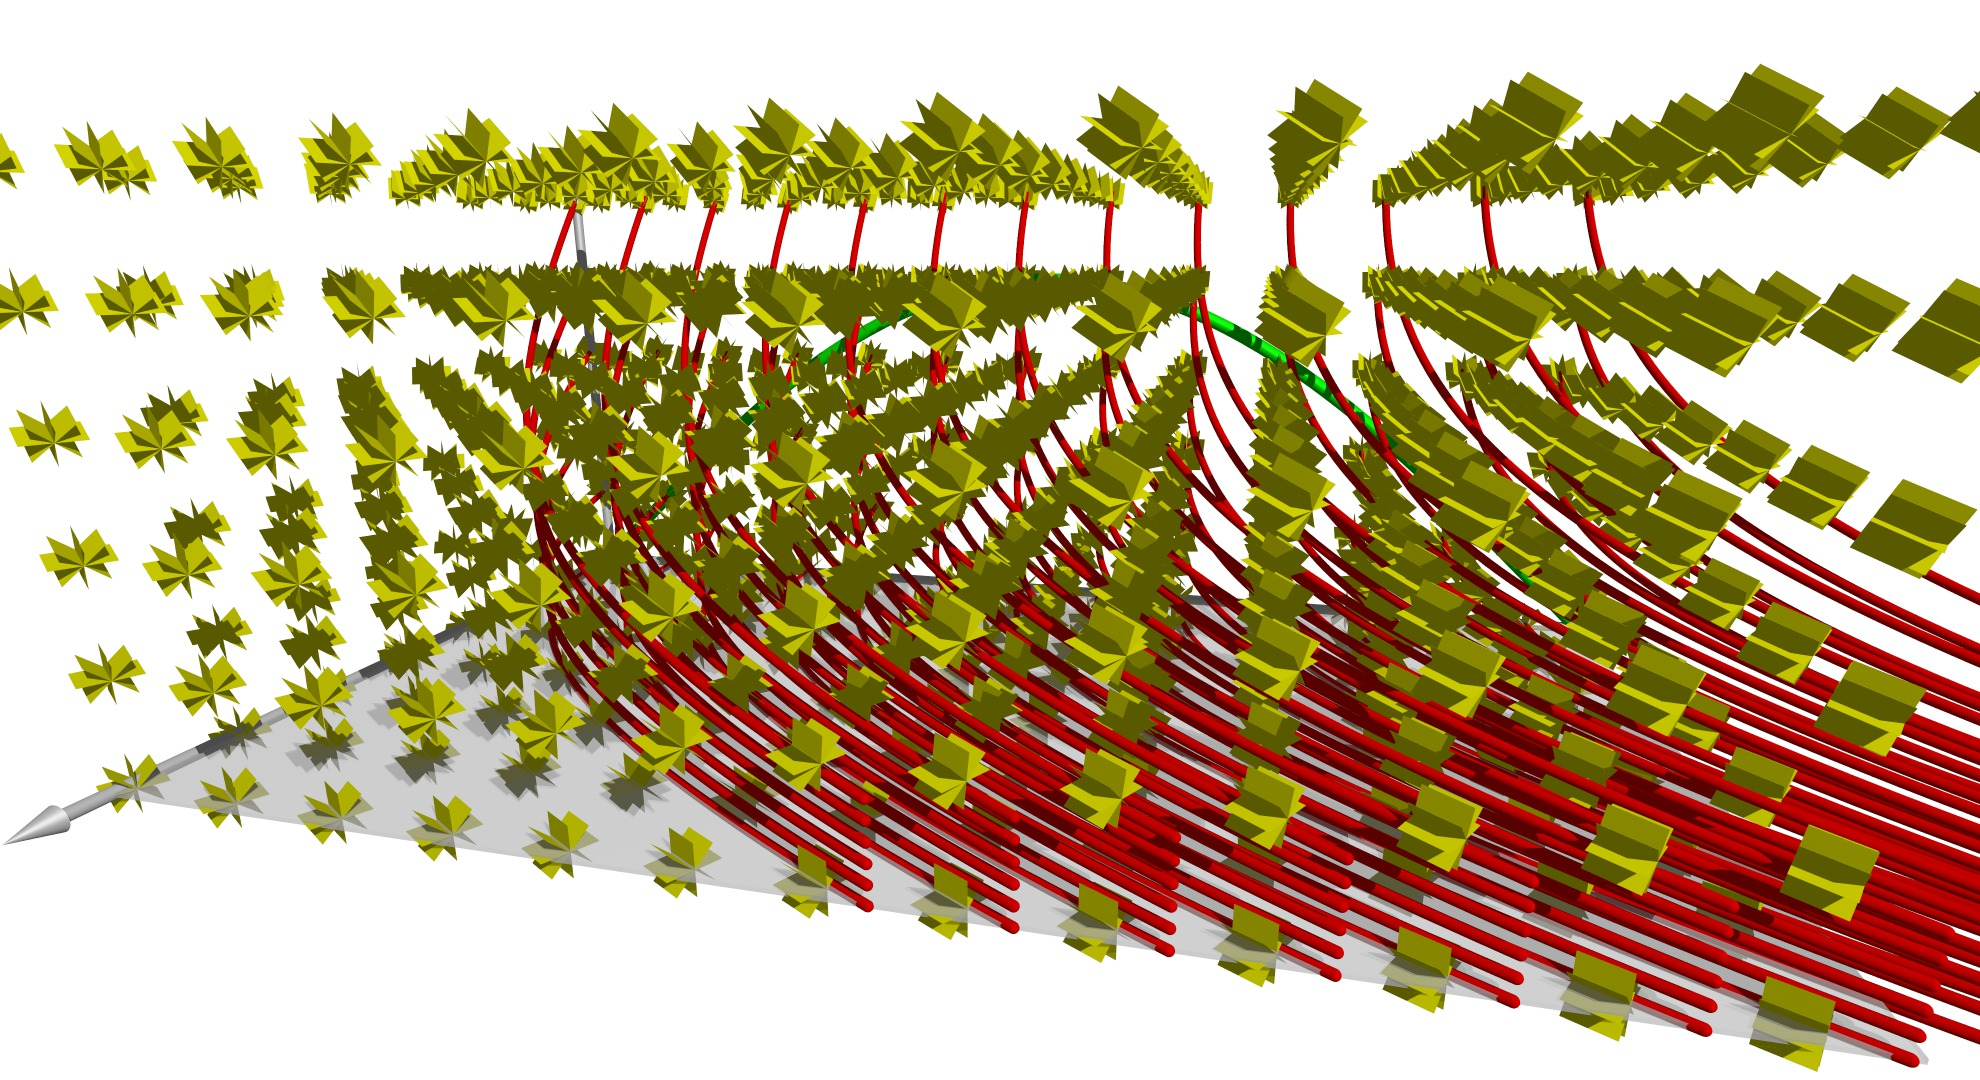
\includegraphics[width=\hsize]{../common/3d/chrpl.jpg}
\end{center}
\begin{center}
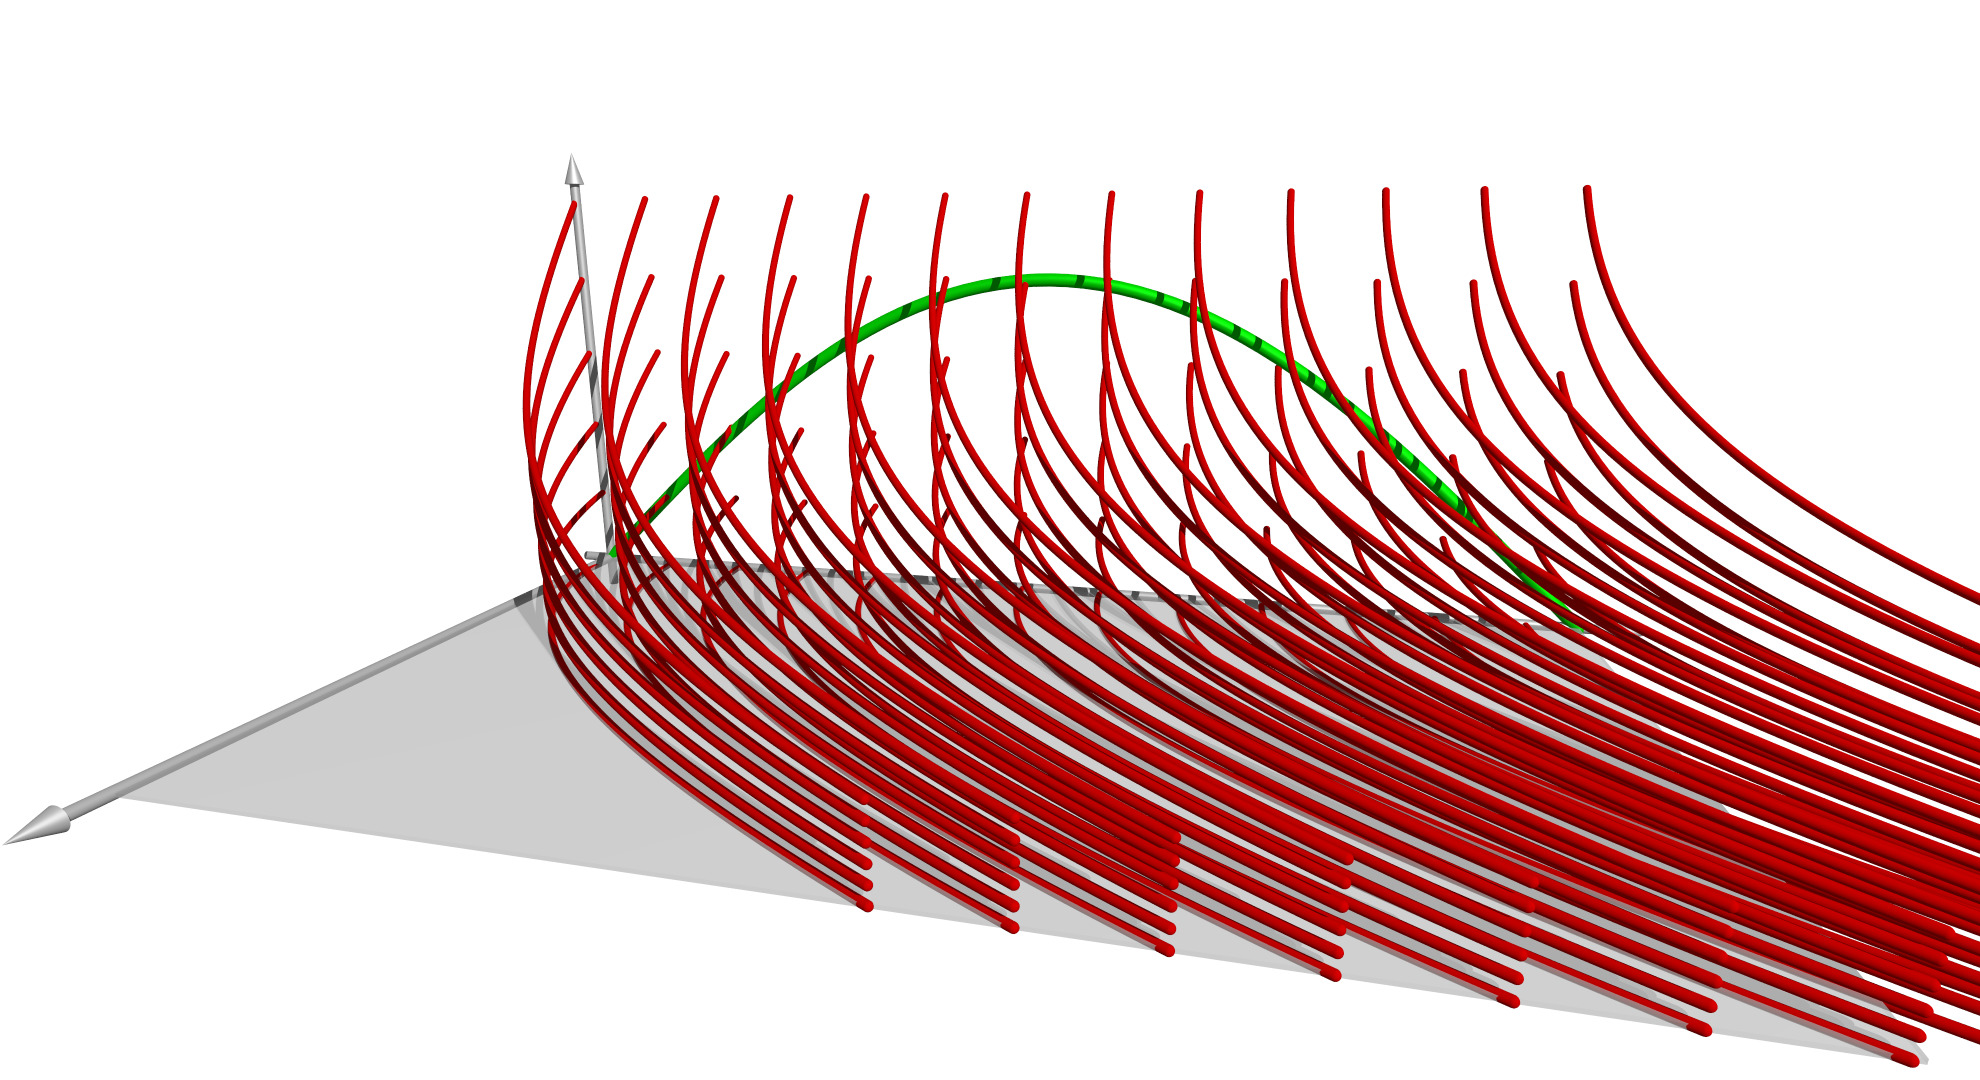
\includegraphics[width=\hsize]{../common/3d/chr.jpg}
\end{center}
\caption{Charakteristiken einer quasilinearen partiellen Differentialgleichung
erster Ordnung, mit eingezeichneten Ebenenbüscheln (oben) und nur die
Charakteristiken (unten)\label{geometrie:charekeristiken-mit-buescheln}}
\end{figure}
Ist ein Punkt der Fläche bekannt,
kann man davon ausgehend eine Lösungskurve des Vektorfeldes konstruieren.
Dazu muss man die gewöhnliche Differentialgleichung
\begin{equation}
\frac{d}{dt}\begin{pmatrix}x(t)\\y(t)\\z(t)\end{pmatrix}
=
\begin{pmatrix}
a(x(t),y(t),u(t))\\b(x(t),y(t),u(t))\\c(x(t),y(t),u(t))
\end{pmatrix}
\label{quasilinear:charakteristik}
\end{equation}
lösen.
Eine Lösungskurve von (\ref{quasilinear:charakteristik}) ist in jedem
Punkt tangential an die Lösungsfläche, sie verlässt die Fläche also
nicht.

\begin{definition}
\label{def:quasiliniear:charakteristik}
\index{Charakteristik!einer quasilinearen partiellen
Differentialgleichung erster Ordnung}
Die Lösungskurven der gewöhnlichen Differentialgleichung
(\ref{quasilinear:charakteristik}) heissen Charakteristiken
der partiellen Differentialgleichung (\ref{quasilinear:equation}).
\end{definition}

\subsubsection{Lösung des Cauchy-Problems}
\begin{figure}
\begin{center}
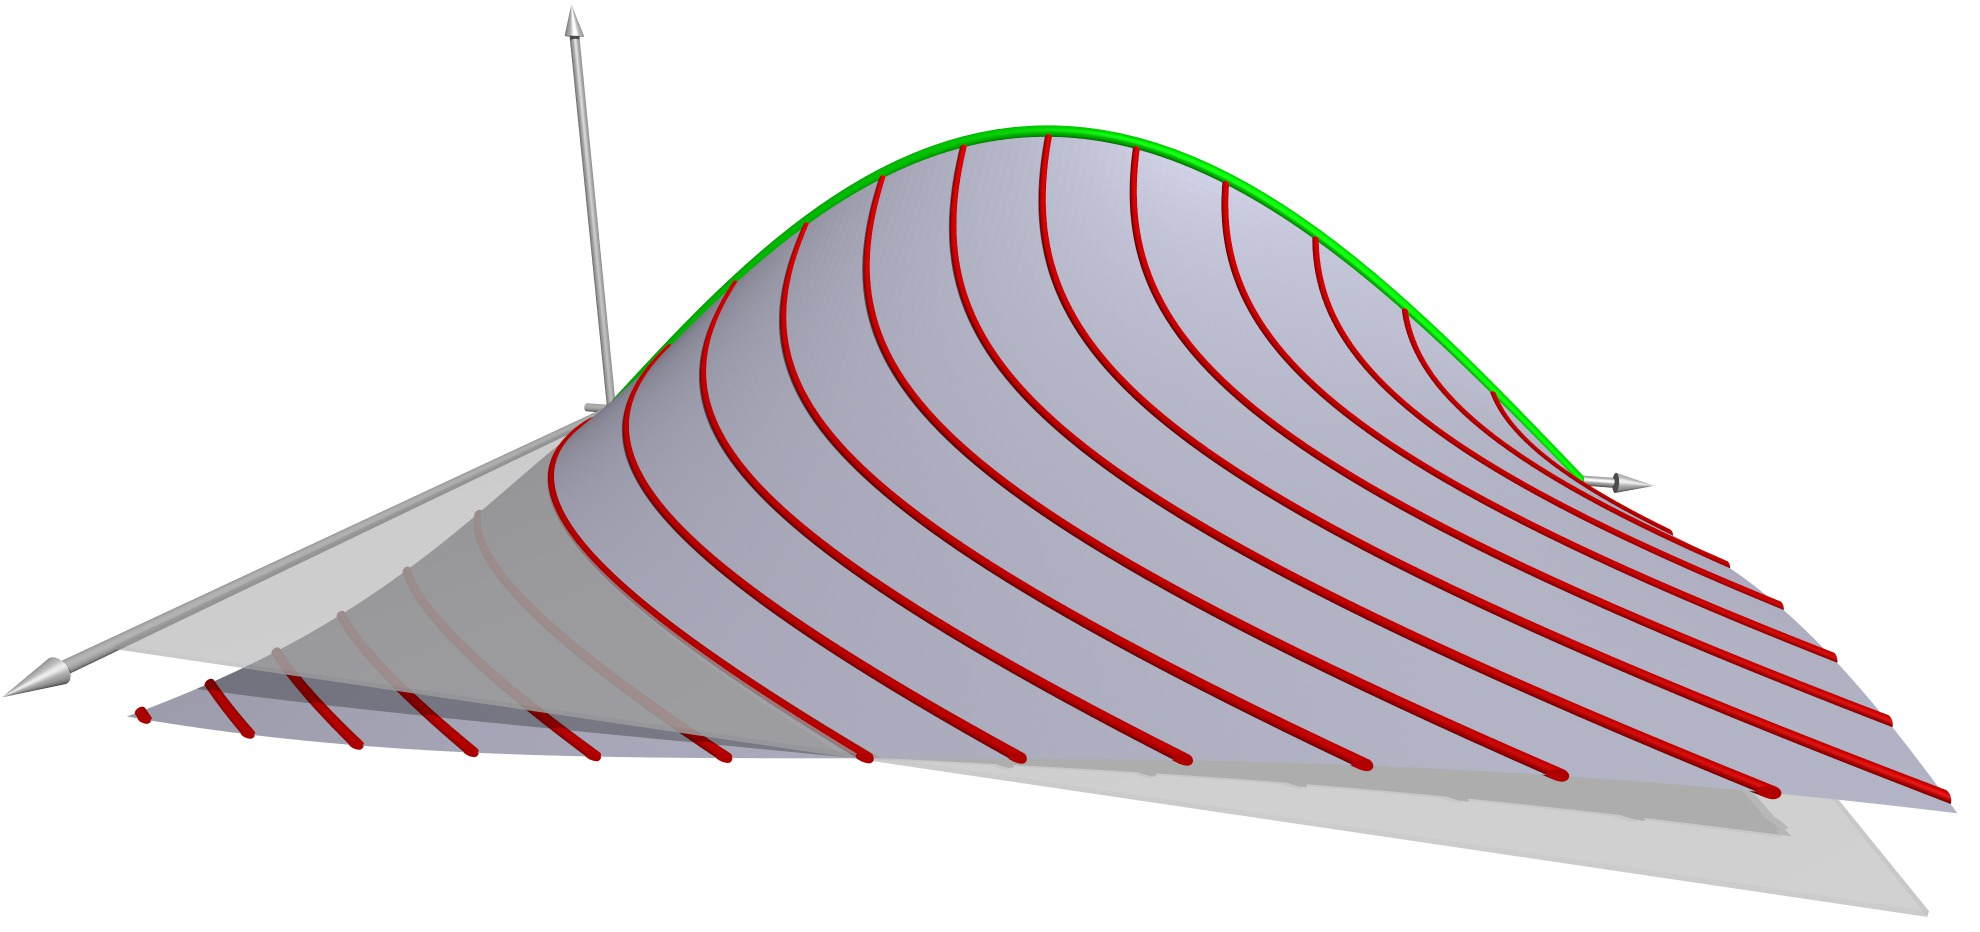
\includegraphics[width=\hsize]{../common/3d/sol.jpg}
\end{center}
\caption{Lösung einer quasilinearen partiellen Differentialgleichung
erster Ordnung: die Lösungsfläche wird von Charakteristiken (rot) gebildet,
sie ist parametrisiert durch den Parameter der Anfangskurve (grün) und den
Kurvenparamter entlang der Charakteristik.
\label{geometrie:loesung-mit-charakteristiken}}
\end{figure}
Das Cauchy-Problem lässt sich jetzt mit Hilfe von Charakteristiken
lösen. Die Lösungsfläche besteht aus Charakteristiken, die auch
die Anfangskurve schneiden
(Abbildung~\ref{geometrie:loesung-mit-charakteristiken}).
Um die Lösung zu berechnen, ist also wie folgt vorzugehen:
\begin{enumerate}
\item
Für jedes $s$ ist die Differentialgleichung der Charakteristiken
(\ref{quasilinear:charakteristik}) zu lösen und eine 
Lösungskurve $t\mapsto \vec x(s,t)$ zu finden, die
die Anfangsbedingung $\vec x(s,0)=\vec x_0(s)$ erfüllt.
\item 
Aus den Gleichungen (\ref{quasilinear:kurvenschar}) für die
Kurvenschar müssen die Parameter $s$ und $t$ eliminiert werden,
sie muss in die Form $z=u(x,y)$ umgeformt werden.
\end{enumerate}

Sind die Koeffizienten der Differentialgleichung differenzierbare Funktionen,
dann ist das Vektorfeld differenzierbar.
Ist auch die Anfangsbedingung differenzierbar,
dann besagen die allgemeinen Sätze über die Abhängigkeit der Lösung einer
gewöhnlichen Differentialgleichung von den Anfangsbedingungen, dass die so
konstruierte Lösungsfläche differenzierbar ist.

Insgesamt haben wir damit das Problem der Lösung der partielle Differentialgleichungen auf das Problem 
zurückgeführt, beliebige Lösungskurven eines Vektorfeldes, also auf
eine gewöhnliche Differentialgleichung zurückgeführt.


\subsubsection{Welche Anfangskurven sind nicht geeignet?}
Damit das eben skizzierte Lösungsverfahren funktioniert, 
darf die Anfangskurve keine Charakteristik sein.
Andernfalls erhält man ja durch Berechnung der von einem Punkt
der Anfangskurve ausgehenden Charakteristik nur wieder die
Anfangskurve, es entsteht gar keine Fläche.

Damit liefern uns die Charakteristiken nicht nur ein Verfahren
zur Lösung einer partiellen Differentialgleichung erster Ordnung,
sondern auch ein Verfahren um zu entscheiden, wo Anfangswerte
vorgegeben werden müssen.

Sei die partielle Differentialgleichung auf dem Gebiet $\Omega$
definiert.
Eine Charakteristik ausgehend von einem Randpunkt mit vorgegebenem
Randwert wird sich zunächst durch das Gebiet bewegen, kann dieses
aber in einem anderen Punkt auch wieder verlassen. Der Wert der
Lösungsfunktion in diesem zweiten Randwert ist offenbar durch die
Vorgabe des ersten Randwertes bereits festgelegt.
Eine andere Vorgabe würde verhindern, dass das Problem überhaupt
eine Lösung hat.

Randwerte müssen also auf einer Teilmenge $M\subset\partial \Omega$
festgelegt werden so, dass jede Charakteristik nur einen Punkt der
Menge $M$ trifft.

\subsection{Beispiele}
In diesem Abschnitt rechnen wir ein paar Beispiel für das eben
skizzierte Lösungsverfahren durch.
\subsubsection{Konstante Koeffizienten\label{konstantekoeff}}
Wir betrachten die Differentialgleichung
\[
\frac{\partial u}{\partial x}+2\frac{\partial u}{\partial y}=3
\]
mit der Anfangsbedingung $u(0,y)=\sin y$ und möchten eine Lösung für
$x>0$ finden.

Die Anfangskurve mit Parameter $s$ hat die Form
\[
\vec x_0(s)
=
\begin{pmatrix}
0\\s\\\sin s
\end{pmatrix}.
\]
Wir müssen also eine Kurvenschar finden, die von dieser Anfangskurve
ausgeht.

Die Differentialgleichung der Charakteristiken ist
\[
\frac{d}{dt}\begin{pmatrix}x(t)\\y(t)\\z(t)\end{pmatrix}
=
\begin{pmatrix}1\\2\\3\end{pmatrix},
\]
sie hat die Lösungskurven
\[
t\mapsto\begin{pmatrix}x_0\\y_0\\z_0\end{pmatrix}+t\begin{pmatrix}1\\2\\3\end{pmatrix}
\]
Der Anfangspunkt $(0,s,\sin s)$ entwickelt sich also mit der Zeit zu
\[
\begin{pmatrix}
x(s,t)\\
y(s,t)\\
z(s,t)
\end{pmatrix}
=
\begin{pmatrix}0\\s\\\sin s\end{pmatrix}+t\begin{pmatrix}1\\2\\3\end{pmatrix}
=
\begin{pmatrix}
t\\
s+2t\\
\sin s+3t
\end{pmatrix}.
\]
Diese Kurvenschar beschreibt die Lösungsfläche, wir möchten daraus aber
wieder die Lösung in der vertrauteren Form $u(x,y)$ gewinnen.
Dazu müssen die Variablen $s$ und $t$ aus den Gleichungen
\begin{align*}
x&=t\\
y&=s+2t\\
z&=\sin s+3t
\end{align*}
eliminiert werden.
Aus der ersten Gleichung folgt, dass $t$ einfach durch $x$ ersetzt werden
kann.
Aus der zweigen Gleichung folgt dann, dass $s=y-2x$.
Setzt man dies in der dritten Gleichung ein, erhält man $z=\sin(y-2x)+3t$.
Die Lösung der Differentialgleichung ist also
\[
u(x,y)=\sin(y-2x)+3x.
\]
Durch Einsetzen in die Differentialgleichung und die Randbedingung
kann man sich davon überzeugen, dass dies tatsächlich eine Lösung
ist:
\begin{align*}
\frac{\partial u}{\partial x}
&=-2\cos(y-2x)+3
\\
\frac{\partial u}{\partial y}
&=\cos (y-2x)
\\
\Rightarrow\qquad
\frac{\partial u}{\partial x}
+2
\frac{\partial u}{\partial y}
&=
-2\cos(y-2x)+3
+2\cos(y-2x)=3
\\
u(0,y_0)&=\sin y_0.
\end{align*}

\subsubsection{Kreisförmige Charakteristiken}
Wir lösen die Differentialgleichung
\[
y\frac{\partial u}{\partial x}-x\frac{\partial u}{\partial y}=0
\]
Gemäss der Methode der Charakteristiken müssen wir die Lösungskurven
des Vektorfeldes
\[
\begin{pmatrix}
y\\-x\\0
\end{pmatrix}
\]
finden. Da die $z$-Komponente verschwindet, sind die $z$-Komponenten
der Lösungskurven konstant, wir ignorieren sie daher in der nachstehenden
Rechnung.

Lösungen für das Vektorfeld 
\[
\begin{pmatrix}
y\\-x
\end{pmatrix}
\]
in der Ebene sind Funktionen $x(t)$ und $y(t)$, welche die Gleichungen
\begin{align*}
\dot x(t)&=y(t)\\
\dot y(t)&=-x(t)
\end{align*}
erfüllen. Leitet man die erste Gleichung ab, und setzt die zweite
darin ein, erhält man die Differentialgleichung zweiter Ordnung
\[
\ddot x(t)=-x(t)
\]
mit den bekannten Lösungen $a\cos t$ und $a \sin t$. Da die Lösungskurve
zur Zeit $t=0$ auf der $y$-Achse beginnen soll, muss sie in Vektorschreibweise
\[
\begin{pmatrix}
x(t)\\y(t)
\end{pmatrix}
=y_0\begin{pmatrix}
\sin t\\
\cos t
\end{pmatrix}
\]
sein, die Kurven sind also Kreise mit Radius $y_0$ um den Nullpunkt. Offenbar
können wir jeden Punkt der Ebene von einem Punkt in der Halbgeraden
$\{(0,y_0)|y_0 <0\}$ aus erreichen, die Anfangsbedingung muss also nur für
$y_0<0$ spezifiziert werden.

Die Lösung zur Anfangsbedingung $g(y)$ kann jetzt wie folgt bestimmt werden.
Zu einem Punkt $(x,y)$ müssen $y_0$ und $t$ gefunden werden, davon brauchen wir
jedoch nur den Betrag, also $y_0=-\sqrt{x^2+y^2}$. Die Lösung ist also
\[
u(x,y)=g(-\sqrt{x^2+y^2}).
\]

Aus diesem Beispiel können wir mehrere Lehren ziehen: 
\begin{enumerate}
\item Dass Festlegung einer Anfangsbedingung für $y_0>0$ nicht nötig ist,
kann man der Differentialgleichung in unmittelbarer Nähe der $y$-Achse nicht
ansehen, erst der Verlauf der Charakterisitiken im Grossen ermöglicht
diese Erkenntnis. Dieses Phänomen wird durch den ``zusätzlichen Platz''
ermöglicht, den der zweidimensionale Definitionsbereich der partielle Differentialgleichung gegenüber dem
eindimensionalen Definitionsbereich der gewöhnlichen DGL bietet.
\item Der Punkt $(0,0)$ hat spezielle Eigenschaften: wenn die Lösung stetig
sein soll, muss $g(0)=\lim_{y\to 0-} g(y)$ sein. Damit die Lösung differenzierbar
wird, muss aber zusätzlich $g'(x)=0$ sein.
\end{enumerate}

\subsubsection{Ein nicht lösbares Anfangswertproblem\label{unloesbar}}
Die Differentialgleichung
\[
x\frac{\partial u}{\partial x}
+
y\frac{\partial u}{\partial y}
=0
\]
soll zu den Anfangsbedingungen $u(0,y)=\sin y$ gelöst werden.
Dazu berechnen wir wieder zuerst die Charakteristiken (ohne die 
$z$-Komponente, die wieder konstant ist)
\[
\frac{d}{dt}
\begin{pmatrix}
x(t)\\y(t)
\end{pmatrix}
=
\begin{pmatrix}
x(t)\\y(t)
\end{pmatrix}
\quad
\Rightarrow
\quad
\left\{
\begin{aligned}
\dot x(t)&=x(t)\\
\dot y(t)&=y(t)
\end{aligned}
\right.
\]
Die Lösungskurven sind Strahlen durch den Ursprung:
\[
\begin{pmatrix}
x(t)\\y(t)
\end{pmatrix}
=\begin{pmatrix}x_0\\y_0\end{pmatrix}e^t
\]
Um die Lösung zu konstruieren, müssen wir jetzt zu einem Punkt
$(x,y)$ den Anfangspunkt der zugehörigen Charakteristik auf der $y$-Achse
finden. Da alle Charakteristiken durch den Nullpunkt gehen, ist dies 
gar nicht möglich. 

Das Problem rührt daher, dass wir die Anfangsbedinung selbst auf einer
Charakteristik festgelegt haben, die Charakteristiken sind also als
Anfangskurven ungeeignet. Nur wenn die Anfangsbedingung auf einer Kurve
festgelegt wird, die transversal, also nirgends tangential, zu den
Charakteristiken verläuft, kann das Anfangswertproblem gelöst werden.

\subsection{Allgemeine partielle Differentialgleichungen erster Ordnung}
Als Beispiel betrachten wir die folgende partielle Differentialgleichung
erster Ordnung für die Funktion $u(x,y)$
\begin{equation}
F\biggl(
x,y,u(x,y),\frac{\partial u}{\partial x},\frac{\partial u}{\partial y}
\biggr)=0.
\end{equation}
Diese Gleichung beschreibt einen impliziten Zusammenhang zwischen
dem Ort im $x$-$y$-$u$-Ko\-or\-di\-na\-ten\-sys\-tem und den beiden Steigungen
$\partial_xu$ und $\partial_yu$.

Ein Anfangswertproblem, bei dem die Anfangswerte für $x=0$ als
Funktion $g(y)$ festgelegt sind, also
\[
u(0,y)=g(y),
\]
legt auch die
partiellen Ableitungen $\partial_y u(0,y)=g'(y)$ fest.  Die partielle
Differentialgleichung schränkt damit ein, welche möglichen Ableitungen
$\partial_xu(0,y)$ möglich sind. Oft wird dies nicht eindeutig sein,
die Steigung in $x$-Richtung kann also verschiedene Werte annehmen,
es kann verschiedene Lösungsfunktionen geben. Ähnlich wie bei der
Lösung gewöhnlicher Differentialgleichungen ist zu jedem Wert
aus der bereits bekannten partiellen Ableitung $\partial_yu(x,y)$
die Steigung $\partial_xu(x,y)$ bestimmt, es ist somit plausibel, dass
sich die Lösung ähnlich wie bei der Lösung gewöhnlicher Differentialgleichungen
entwickeln lässt. In voller Allgemeinheit ist dies nicht ganz einfach,
und für unsere Zwecke auch nicht notwendig, denn alle wesentlichen
Eigenschaften lassen sich an dem einfacheren Fall der quasilinearen
partielle Differentialgleichung auch beobachten.



%
% singularities.tex -- XXX
%
% (c) 2019 Prof Dr Andreas Mueller, Hochschule Rapperswil 
%
\section{Entstehung von Singularitäten\label{burgersunstetig}}
\rhead{Singularitäten}
\begin{figure}
\begin{center}
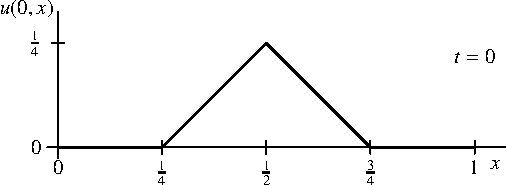
\includegraphics[width=0.8\hsize]{../common/images/burgers-1}
\end{center}
\caption{Anfangsbedingung für die Burgers Gleichung einer idealen
Flüssigkeit\label{burgersanfang}}
\end{figure}
In diesem Abschnitt möchten wir die Burgers Gleichung für die ideale
Flüssigkeit
\[
\frac{\partial}{\partial t}u+\frac{\partial}{\partial x}\left(\frac{u^2}2\right)=0
\]
auf dem Interval $x\in[0,1]$ und für $t>0$
mit der Anfangsbedingung
\[
u(0,x)=\begin{cases}
0\qquad&\text{$x<\frac14$ oder $x>\frac34$}\\
x-\frac14\qquad&\frac14\le x\le \frac12\\
\frac34-x\qquad&\frac12\le x\le \frac34
\end{cases}
\]
lösen (siehe Abbildung \ref{burgersanfang}).

\begin{figure}
\begin{center}
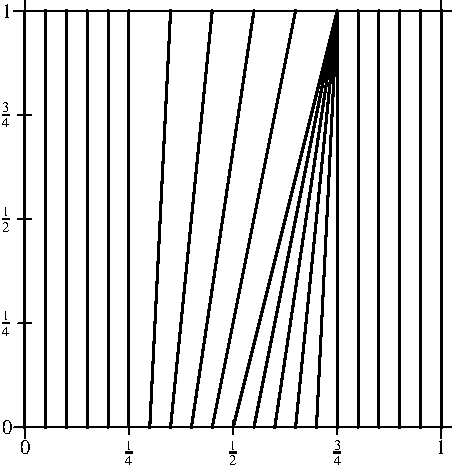
\includegraphics[width=0.8\hsize]{../common/images/burgers-2}
\end{center}
\caption{Niveaulinien (Charakteristiken) der Lösung der Burgers-Gleichung für
die ideale Flüssigkeit\label{burgersniveau}}
\end{figure}
Die Differentialgleichung ist von erster Ordnung, in der Form
\[
\partial_tu+u\partial_xu=0
\]
haben wir die zugehörige geometrische Theorie in Abschnitt
\ref{pdgl1ordnung} besprochen. Dort wurde darauf hingewiesen,
dass der Vektor 
\[
\begin{pmatrix}
1\\u\\0
\end{pmatrix}
\]
immer an die Fläche $u=u(t,x)$ tangential ist. Die Lösungsfläche
entsteht dadurch, dass die Anfangsbedingung mit Hilfe dieses Vektors
verschoben wird. 
Der Punkt $(0,x,u(0,x))$ entwickelt sich nach dieser Methode zu
Punkten $(t,x+u(0,x)t, u(0,x))$ der Lösungsfläche. Die Kurven
gleichen Funktionswertes bilden also Geraden, deren Steigung im
$x$-$t$-Koordinatensystem $u(0,t)^{-1}$ ist. Die Niveaulinien der
Lösung sehen daher aus wie in der Abbildung \ref{burgersniveau}
dargestellt.
Daraus kann man jetzt auch die Lösungen ablesen. In der Abbildung
\ref{burgerssprung} kann man die Entwicklung der Spitze zu einem
Sprung an der Stelle $x=\frac34$ beobachten.

\begin{figure}
\begin{center}
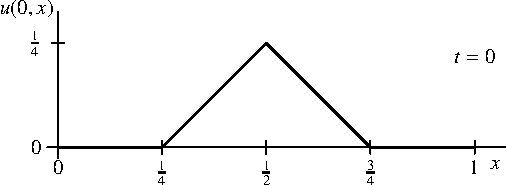
\includegraphics[width=0.8\hsize]{../common/images/burgers-1}
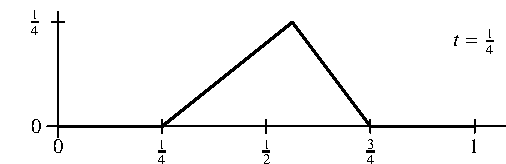
\includegraphics[width=0.8\hsize]{../common/images/burgers-3}
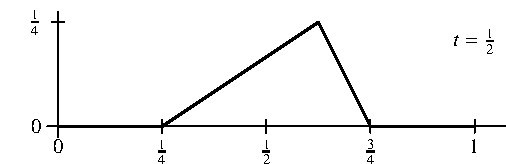
\includegraphics[width=0.8\hsize]{../common/images/burgers-4}
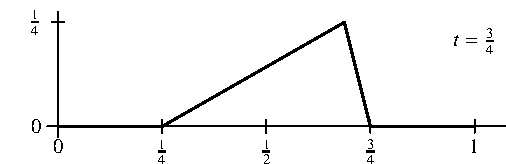
\includegraphics[width=0.8\hsize]{../common/images/burgers-5}
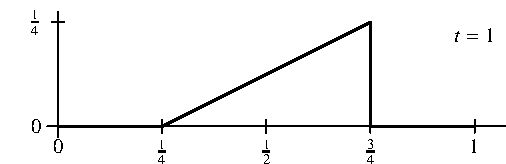
\includegraphics[width=0.8\hsize]{../common/images/burgers-6}
\end{center}
\caption{Entwicklung eines Sprungs in der Lösung der Gleichung von Burgers\label{burgerssprung}}
\end{figure}

Man könnte argumentieren, dass die Anfangsbedingung ja bereits nicht differenzierbar
ist, und dass die Lösungen dies ebenfalls nicht sind. Man kann
jedoch eine beliebige glatte Funktion als Anfangsbedingung wählen, welche
innerhalb des Intervals $[\frac14,\frac12]$ monoton von $0$ auf $\frac14$ 
ansteigt, im Punkt $x=\frac12$ den maximalen Wert $\frac14$ annimmt,
und im Interval $[\frac12,\frac34]$ monoton auf $0$ abfällt.
Das Maximum wird sich entlang der Charakteristiken zum Punkt
$(1,\frac34,\frac14)$ entwicklen. Der Funktionswert $u(0,x)$ im Punkt $(0,x)$
für $x\in[\frac14,\frac12]$ ist derselbe wie im Punkt $(1,x+u(0,x))$.
Der Funktionsgraph $x\mapsto u(1,x)$ hat also die Parameterdarstellung
\[
[{\textstyle\frac14},{\textstyle\frac12}]\to\mathbb R\colon s\mapsto (s+u(0,s),u(0,s))
\]
Diese ist jedenfalls eine glatte Funktion. Andererseits komprimieren
die Charakteristiken das Interval $[\frac12,\frac34]$ auf
den Punkt $(1,\frac34)$ so dass bei $x=\frac34$ wieder ein Sprung entsteht.


%
% boundry.tex  -- 
%
% (c) 2019 Prof Dr Andreas Mueller
%
\section{Boundary conditions}
The method of characteristics allows us to find out on which parts of the
boundary we have to specify boundary conditions to make the solution
unique.
The solution surface corresponding to $u(x,y)$ consists of characteristics
so it is uniquely determined if exactly one characteristic goes through
each point.

For the differential equation
\begin{equation}
\frac{\partial u}{\partial x}+2\frac{\partial u}{\partial y}=3
\label{geometrie:knickbeispiel}
\end{equation}
we have found the characteristics
\[
t\mapsto\begin{pmatrix}x_0\\y_0\\z_0\end{pmatrix}+t\begin{pmatrix}1\\2\\3\end{pmatrix}.
\]
The graph of the solution function $u(x,y)$ must be covered by characteristics.
The projections of these curves into the $x$-$y$-plane are straight lines
with slope $2$.
The boundary of the domain $\Omega$, in which the equation needs to be
solved, thus must intersect each straight line with slope $2$ exactly once.

The domain
$\{(x,y)\in\mathbb R^2\,|\, x >0\}$  from \ref{konstantekoeff}
has the $x$-axis as boundary which intersects every straight line with
slope exactly once.

The domain $\Omega=\{(x,y)\,|\,0<x,y<1\}$ is more interesting.
Figures \ref{geometrie:charrand1}
to \ref{geometrie:charrand3}
show various possibilities:
\begin{enumerate}
\item
In figure~\ref{geometrie:charrand1}
boundary values are prescribed on the left and right boundary.
These boundary values are not sufficient to determine the solution
everywhere in the domain.
There is a part not covered by characteristics where the solution
is not fixed.
\item
In figure~\ref{geometrie:charrand2}
boundary values are given on the top and bottom boundaries of the
square.
A solution is only possible if the values solution emanating from
the left half of the bottom boundary coincides with the solution
emanating from the right half of the top boundary.
If the boundary values on these parts are not compatible, no solution
exists.
\item
In figure~\ref{geometrie:charrand3}
the boundary values are specified on the left and bottom side
of the square.
This fixes the solution function uniquely.
Nevertheless it is not entirely clear that we have found a solution,
because it is still possible that the combined function is not
differentiable on the characteristic through the lower left
corner of the square.
\end{enumerate}
The last situation is very common, the solution we find here is
differentiable outside of a set of measure zero.
This is called a {\em weak} solution of the differential equation.

\begin{figure}
\begin{center}
\includegraphics{../common/images/randwerte-2.pdf}
\end{center}
\caption{Boundary values on the left and right side: solution
not determined in the light green portion of the domain.
\label{geometrie:charrand1}}
\end{figure}

\begin{figure}
\begin{center}
\includegraphics{../common/images/randwerte-3.pdf}
\end{center}
\caption{Boundary values on the top and bottom side of the square:
solution overdetermined in the light green portioin of the domain
\label{geometrie:charrand2}}
\end{figure}

\begin{figure}
\begin{center}
\includegraphics{../common/images/randwerte-4.pdf}
\end{center}
\caption{Boundary values on the left and bottom sides of the square:
solution well defined but differentiability on the light green
characteristic emanating from $(0,0)$ is not guaranteed.
\label{geometrie:charrand3}}
\end{figure}

\begin{figure}
\centering
\includegraphics[width=\hsize]{../common/3d/knick.jpg}
\caption{The solution of the differential
equation~(\ref{geometrie:knickbeispiel}),
with boundary values along the left and bottom sides of the square
(see also figure~\ref{geometrie:charrand3})
is not differentiable along the characteristic through $(0,0)$
(vertical axis scaled by a factor $0.4$).
\label{geometrie:knick}}
\end{figure}

As an illustration of the last case consider the boundary values
\begin{align*}
u(x_0,0)&=0,\\
u(0,y_0)&=y_0.
\end{align*}
Each side fixes part of the solution in the unit square, we can get 
explicit formulas using the method of characteristics.
The characteristics starting from the bottom side are
\[
\left.
\begin{aligned}
x&=x_0+t\\
y&=2t\\
u&=3t
\end{aligned}
\right\}
\qquad\Rightarrow\qquad
\left\{
\begin{aligned}
t&=\frac12y\\
u&=\frac32y
\end{aligned}
\right.
\]
The characteristics from the left side of the square are
\[
\left.
\begin{aligned}
x&=t\\
y&=y_0+2t\\
u&=y_0+3t
\end{aligned}
\right\}
\qquad\Rightarrow\qquad
\left\{
\begin{aligned}
y_0&=y-2x\\
u&=y+x
\end{aligned}
\right.
\]
Thus the solution function is
\[
u(x,y)=\begin{cases}
\frac32y&\qquad y<2x\\
x+y&\qquad y>2x,
\end{cases}
\]
as displayed in figure~\ref{geometrie:knick}.
For $y=2x$, both terms coincide, so the solution function is continuous
in all of $\Omega$.
However, the partial function $x\mapsto u(x,y)$ has slope $1$
for $y>2x$ and slope $0$ for $y<2x$, so it is not differentiable at $y=2x$.


%
% higher.tex - QLPDE in higher dimensions
%
% (c) 2021 Prof Dr Andreas Müller, OST Ostschweizer Fachhochschule
%
\section{Higher dimensions
\label{geometry:section:higher-dimensions}}
\rhead{Higher dimensions}
The very geometric principles used to solve a quasilinear
partial differential equation of first order also works in higher
dimensions.

\subsection{Differential equation in dimension $n$}
A quasilinear partial differential equation of $n$ variables $x_1,\dots,x_n$
is of the form
\begin{equation}
a_1(x_1,\dots,x_n,u) \frac{\partial u}{\partial x_1}
+
a_2(x_1,\dots,x_n,u) \frac{\partial u}{\partial x_2}
+
\dots
+
a_n(x_1,\dots,x_n,u) \frac{\partial u}{\partial x_n}
=
c(x_1,\dots,x_n,u)
\label{qlpden:eqn:equation}
\end{equation}
where the coefficients $a_1$ to $a_n$ and $c$ are functions
depending on the variables $x_1,\dots,x_n$ and the function $u$.
If they do not depend on $u$, then the equation is actually linear.

The equation~\eqref{qlpden:eqn:equation} is defined on the domain
$\Omega\subset\mathbb{R}^n$.
For brevity, we will write the points $(x_1,\dots,x_n)\in \Omega$
as just $x\in\Omega$.

In addition, we need some boundary conditions in the form
$
u(x) = f(x) 
$
for points $x$ in some part of the boundary $\partial\Omega$.
To compute the solution using the method of characteristics, we need to
parametrize the part of the boundary, an $n-1$-dimensional surface, using 
a function
\begin{equation}
s=(s_1,\dots,s_{n-1})
\mapsto
\xi(s_1,\dots,s_{n-1}) = \xi(s) \in \partial\Omega.
\end{equation}
The parameters $s=(s_1,\dots,s_{n-1})$ come from a subset
$S\subset\mathbb{R}^{h-1}$.
The boundary conditions for the function $u$ can then be written as
\begin{equation}
u(\xi(s)) = f(\xi(s))
\end{equation}
for all $s\in S$.
The boundary surface is an $n-1$-dimensional hypersurface of the
$n$-dimensional space of the variables $x_1,\dots,x_n$.

\subsection{Solution as a graph}
The solution of the partial differential equation~\eqref{qlpden:eqn:equation}
is a function  $u(x_1,\dots,x_n)$.
This function describes an $n$-dimensional hypersurface in the
$n+1$-dimensional space with
variables $(x_1,\dots,x_n,z)\in\mathbb{R}^{n+1}$ consisting of all the
points of the form $(x_1,\dots,x_n,u(x_1,\dots,x_n))$.

The boundary conditions also have a geometric description.
For points $x$ on the boundary part for which we have boundary conditions,
$u(x)=f(x)$.
This means that the $n$-dimensional surface specified by
$(x_1,\dots,x_n,u(x))$ has to pass through the points of the $n-1$-dimensional
surface of points $(x_1,\dots,x_n,f(x))$ where $x$ is in the relevant
part of the boundary.
Using the parametrization, the $n-1$-dimensional boundary surface is
parametrized by $S$ via the function
\[
S\to \mathbb{R}^n
:
s\mapsto (\xi_1(s), \dots,\xi_n(s), f(\xi(s))).
\]
This is the generalized formulation of the Cauchy-Problem.

\subsection{Characteristics}
As in the two-dimensional situation for $n=2$, the differential
equation \eqref{qlpden:eqn:equation} can be interpreted as the
vector equation
\[
\underbrace{
{\color{red}
\begin{pmatrix}
a_1(x_1,\dots,x_n,u)\\
\vdots \\
a_1(x_1,\dots,x_n,u)\\
c(x_1,\dots,x_n,u)
\end{pmatrix}
}}_{\displaystyle = \vec{v}}
\cdot
\begin{pmatrix}
\frac{\partial u}{\partial x_1}\\
\vdots \\
\frac{\partial u}{\partial x_n}\\
-1
\end{pmatrix}
=
0.
\]
The vector on the left was previously called $\vec{v}$ and was usually
shown in {\color{red}red}.
The vector on the right is again the normal vector on the $n$-dimensional
hypersurface defined by $u$.
To understand this, we have to look at the the function
$
g(x,z) = u(x) - z.
$
The graph of $u$ is the set of points such that $g(x,z) = 0$.
The normal to this surface is obtained by taking the gradient of $g$ in
this $n+1$-dimensional space, i.~e.
\begin{equation}
\vec{n}
=
\operatorname{grad} g
=
\begin{pmatrix}
\frac{\partial g}{\partial x_1}\\
\vdots \\
\frac{\partial g}{\partial x_n}\\
\frac{\partial g}{\partial z}
\end{pmatrix}
=
\begin{pmatrix}
\frac{\partial u}{\partial x_1}\\
\vdots \\
\frac{\partial u}{\partial x_n}\\
-\frac{\partial z}{\partial z}
\end{pmatrix}
=
\begin{pmatrix}
\frac{\partial u}{\partial x_1}\\
\vdots \\
\frac{\partial u}{\partial x_n}\\
-1
\end{pmatrix}.
\end{equation}
The geometric content of the partial differential equation thus is that
$\vec{v}(x_1,\dots,x_n,z)\perp \vec{n}(x_1,\dots,x_n,u)$ for all points
on the solution surface.

Following the ideas of the two-dimensional case we conclude that a
curve that always has $\vec{v}$ as a tangent vector will be contained
in the solution surface.
These curves can be parametrized using some parameter $t$ and written
as functions
\begin{equation}
x(t)
=
\begin{pmatrix}
x_1(t)\\
\vdots\\
x_n(t)
\end{pmatrix}.
\label{qlpden:charparam}
\end{equation}
They are solutions of the ordinary differential equations
\begin{equation}
\frac{d}{dt}
\begin{pmatrix}
x_1(t)\\
x_2(t)\\
\vdots\\
x_n(t)\\
z(t)
\end{pmatrix}
=
\begin{pmatrix}
a_1(x_1(t),\dots,x_n(t),z(t))\\
a_2(x_1(t),\dots,x_n(t),z(t))\\
\vdots \\
a_n(x_1(t),\dots,x_n(t),z(t))\\
c(x_1(t),\cdots,x_n(t),z(t))
\end{pmatrix}.
\label{qlpden:chareqn}
\end{equation}
The curves should all begin on the $n-1$-dimensional boundary surface,
so the initial values of the functions $x_i(t)$ and $z(t)$ für $t=0$ 
must be given by $f$ in the form
\begin{equation}
\begin{aligned}
x_1(0) &= \xi_1(s)
\\
x_2(0) &= \xi_2(s)
\\
&\phantom{i}\vdots
\\
x_n(0) &= \xi_n(s)
\\
z(0) &= f(\xi(s)),
\end{aligned}
\label{qlpden:initial}
\end{equation}
where $s\in S$ is the $n-1$-dimensional parameter that parametrizes the
boundary.

\subsection{Solution}
To solve the partial differential equation, we first have to solve
the ordinary differential equations~\eqref{qlpden:chareqn} with the
initial conditions~\eqref{qlpden:initial}.
The solution curves will depend on the parameters $s_1,\dots,s_{n-1}$ 
of the boundary, so we will get a curve parametrization $x(t,s)$
with coordinates
$x_i(t,s_1,\dots,s_{n-1})$
satisfying the differential equations
\begin{align*}
\frac{d}{dt}
x_i(t,s_1,\dots,s_{n-1})
&=
a_i(x(t,s_1,\dots,s_{n-1}), z(t))
\\
\frac{d}{dt}
z(t,s_1,\dots,s_{n-1})
&=
c(x(t,s_1,\dots,s_{n-1}),z(t))
\end{align*}
with the initial conditions
\begin{align*}
x_i(0,s_1,\dots,s_{n-1})
&=
\xi(s_1,\dots,s_{n-1})
\\
z(0,s_1,\dots,s_{n-1})
&=
f(\xi(s_1,\dots,s_{n-1}))
\end{align*}
at $t=0$.

Now we have to turn the functions $x_i$ and $z$ into a function
$u(x_1,\dots,x_n)$.
The equations
\[
\begin{aligned}
x_i &= x_i(t,s_1,\dots,s_{n-1}) &\qquad 1\le i \le n
\\
  u(x_1,\dots,x_n) &= z(t,s_1,\dots,s_{n-1})
\end{aligned}
\]
are $n+1$ equations with variables $x_i$, $t$, $s_j$ and $u$,
i.~e.~$n+1+(n-1)+1=2n+1$ variables.
By inverting the first $n$ equations and expressing the parameters
$t,s_1,\dots,s_n$ in terms of $x_1,\dots,x_n$, we can eliminate the
parameters by substiting them into the function $z$.
This gives the solution function in the form $u(x_1,\dots,x_n)$.

\subsection{Well-posedness}
The method of characteristics was also used in the two-dimensional 
case to decide whether the specified boundary conditions uniquely
determine the solution.
The problem is well posed if the characteristics that emanate from
the Cauchy initial curve cover all of the domain exactly once.
Similarly, the problem in $n$ dimensions is well posed if the
for each point $x\in\Omega$ there is precisely one boundary point
and boundary value such that the characteristic starting at this
boundary value passes over the point $x$, and the value of the
solution is the $z$-coordinate of the characteristic when it passes
over $x$.

\subsection{Examples}
\subsubsection{An equation on a a half space}
Find the solution of the equation
\[
\frac{\partial u}{\partial x_1}
+
2x_1
\frac{\partial u}{\partial x_2}
+
3
\frac{\partial u}{\partial x_3}
=
0
\]
in the half space
\[
\Omega
=
\{
(x_1,x_2,x_3)
\,|\,
x_3>0
\}
\]
with boundary values
\begin{align*}
u(x_1,x_2,0) = f(x_1,x_2)
\end{align*}
for $x_2,x_3\in\mathbb{R}$.

The differential equations for the characteristics are
\begin{align*}
\dot{x}_1 &= 1    &&\Rightarrow&  x_1(t) &= t + s_1                 \\
\dot{x}_2 &= 2x_1 &&\Rightarrow&  x_2(t) &= t^2 + 2s_1t + s_2        \\
\dot{x}_3 &= 3    &&\Rightarrow&  x_3(t) &= 3t                      \\
\dot{u}   &= 0    &&\Rightarrow&  u(t)   &= f(s_1,s_2)
\end{align*}
From these equations, we have to eliminate $t$, $s_1$ and $s_2$.
The third equation tells us that $x_3=3t$, which eliminates $t$:
\begin{align*}
x_1 &= \frac13x_3 + s_1                   \\
x_2 &= \frac1{9}x_3^2 + \frac{2s_1x_3}3 + s_2 \\
u   &= f(s_1,s_2).
\end{align*}
The first equation is equivalent to $s_1=x_1-\frac13x_3$,
which eliminates $s_1$:
\begin{align*}
x_2
&=
\frac1{9}x_3^2 + \biggl(x_1-\frac{x_3}3\biggr)\frac{2x_3}3 + s_2
=
-\frac{x_3^2}{9}
+
\frac{2x_1x_3}{3} + s_2\\
u   &= f\biggl(x_1-\frac13x_3,s_2\biggr).
\end{align*}
The equation for $x_2$ can be solved for
\[
s_2
=
x_2+\frac{1}{9}x_3^2-\frac{2x_1x_3}3
\]
and substituted into the expression for $u$ which gives the solution
\begin{equation}
u(x_1,x_2,x_3)
=
f\biggl(x_1-\frac13x_3, x_2+\frac{1}{9}x_3^2-\frac{2x_1x_3}{3}\biggr).
\label{qlpden:ex1solution}
\end{equation}
To verify this solution, we compute the partial derivatives
\begin{align*}
\frac{\partial u}{\partial x_1}
&=
\frac{\partial f}{\partial s_1}
-\frac{2x_3}{3}
\frac{\partial f}{\partial s_2}
\\
\frac{\partial u}{\partial x_2}
&=
\frac{\partial f}{\partial s_2}
\\
\frac{\partial u}{\partial x_3}
&=
-
\frac{1}{3}
\frac{\partial f}{\partial s_1}
+
\biggl(
\frac{2}{9}x_3-\frac{2x_1}{3}
\biggr)
\frac{\partial f}{\partial s_2}
\end{align*}
and substitute them into the partial differential equation
\begin{align*}
\frac{\partial u}{\partial x_1}
+
2x_1\frac{\partial u}{\partial x_2}
+
3
\frac{\partial u}{\partial x_3}
&=
\biggl(
\frac{\partial f}{\partial s_1}
-\frac{2x_3}3
\frac{\partial f}{\partial s_2}
\biggr)
+2x_1
\frac{\partial f}{\partial s_2}
+
3
\biggl(
-
\frac{1}{3}
\frac{\partial f}{\partial s_1}
+
\biggl(
\frac{2x_3}{9}
-\frac{2x_1}{3}
\biggr)
\frac{\partial f}{\partial s_2}
\biggr)
\\
&=
\biggl(
1-3\cdot\frac13
\biggr)
\frac{\partial f}{\partial s_1}
+
\biggl(
-\frac{2x_3}{3}
+
2x_1
+
3\cdot \frac{2}{9}x_3
-3\cdot\frac{2x_1}{3}
\biggr)
\frac{\partial f}{\partial s_2}
=0.
\end{align*}
So \eqref{qlpden:ex1solution} is in fact the solution of the equation.

\subsubsection{An analog to Burgers equation in three dimensions}
We want to solve the equation
\begin{equation}
u\biggl(
\frac{\partial u}{\partial x_1}
+
\frac{\partial u}{\partial x_2}
+
\frac{\partial u}{\partial x_3}
\biggr)
=
0
\end{equation}
which is clearly quasilinear and of first order.
We want tos olve it in the domain
\[
\Omega
=
\{ (x_1,x_2,x_3) \,| x_3>0\},
\]
the boundary of which is the $x_1$-$x_2$-plane which we can parametrize
using the $s_1=x_1$ and $s_2=x_2$ with with the function
\[
\xi(s)
=
\begin{pmatrix}
s_1\\
s_2\\
0
\end{pmatrix}.
\]
The boundary values are given by a function $f(x_1,x_2)$.

The system of ordinary differential equations for the characteristics is
\begin{align*}
\dot{x}_1 &= z &&\Rightarrow& x_1(t) = zt + s_1
\\
\dot{x}_2 &= z &&\Rightarrow& x_2(t) = zt + s_2
\\
\dot{x}_3 &= z &&\Rightarrow& x_3(t) = zt
\\
\dot{z} &= 0 &&\rightarrow& z = f(s_1,s_2)
\end{align*}
where we have already substituted the boundary conditions.
We now have to eliminate the variables $t$, $s_1$ and $s_2$ from the
equations
\[
\begin{aligned}
x_1 &= f(s_1,s_2)t + s_1 \\
x_2 &= f(s_1,s_2)t + s_2 \\
x_3 &= f(s_1,s_2)t       \\
u(x_1,x_2,x_3) &= f(s_1,s_2).
\end{aligned}
\]
The first three equations describe a straight line
in the domain
through the point
\[
\vec{p}
=\begin{pmatrix}
s_1\\s_2\\0
\end{pmatrix}
\]
with direction vector
\[
\vec{r}
=
f(s_1,s_2)
\begin{pmatrix} 
1\\1\\1
\end{pmatrix}.
\]
which establishes the similarity to the solution of Burgers equation
we have investigated previously.
In particular, the $3$-dimensional solution surface is covered by straight
lines
of the form
\[
\begin{pmatrix}
x_1\\
x_2\\
0\\
f(x_1,x_2)
\end{pmatrix}
+
f(x_1,x_2)\begin{pmatrix}1\\1\\1\\0\end{pmatrix}.
\]


\section{Summary}
\begin{enumerate}
\item
The generalization of direction field from the theory of ordinary
differential equations is a sheaf of planes.
The graph of the solution function must have a tangent plane in the 
sheaf for every point.
\item
The planes of the sheaf have a common vector, called the axis of the sheaf,
or informally in these notes the ``red'' vector.
\[
\begin{pmatrix}
a(x,y,u)\\
b(x,y,u)\\
c(x,y,u)
\end{pmatrix}.
\]
Integral curves of this vector field are called characteristics
or informally ``red'' curves.
\item
The solution surface of a quasilinear partial differential equation
is covered by characteristics that all go through the initial curve
(informally the ``green'' curve).
\item
To find the solution function, eliminate the parameter of the initial
curve and the of the characteristics.
\item
Characteristics are those curves that are not suitable as initial
curves.
This characterization will become even more useful in
chapter~\ref{chapter:hyperbolic}.
\item
With the help of characteristics it is possible to decide which boundary
conditions are necessary in order for a problem to be well posed.
\end{enumerate}
